\section{Versuchsaufbau und Versuchsdurchführung}

\begin{figure}[H]     
    \centering
    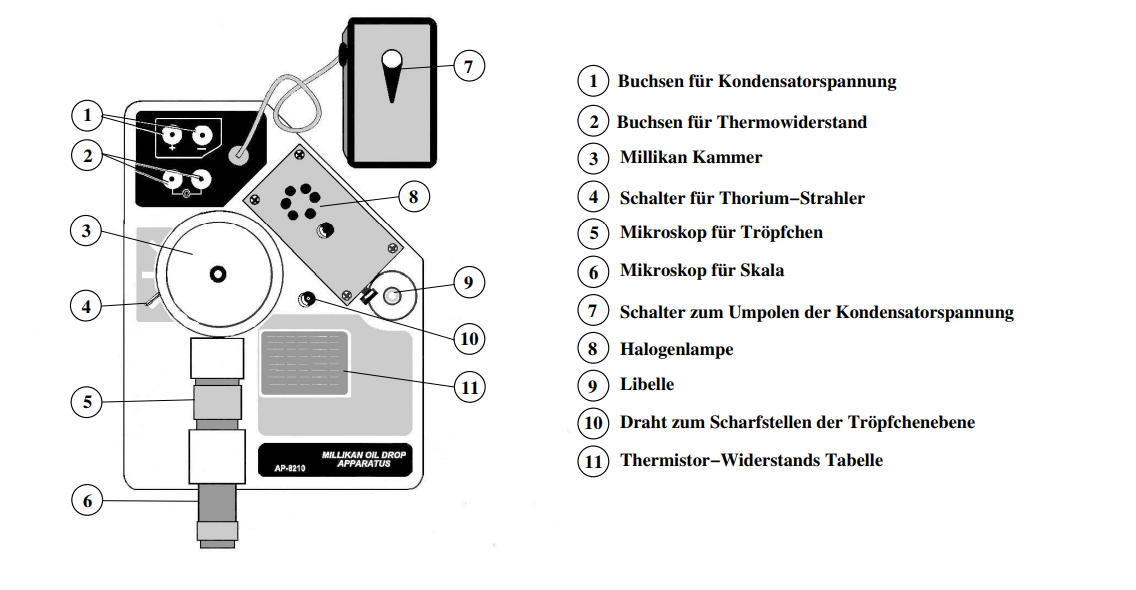
\includegraphics[height=80mm]{bilder/Abb2.png}
    \caption{ Apparatur zum Millikan-Öltröpfchenversuch \cite{a1}. \label{Abbildung2} }
\end{figure}

\begin{flushleft}
    Der Versuch wird mit der Apparatur aus Abbildung \ref{Abbildung2} durchgeführt, welcher mit einer Spannungsquelle verbunden ist.
    Optional kann vorne an das Mikroskop eine Kamera angebracht werden, welche mit einem Monitor verbunden ist für ein einfacheres Beobachten.
    Zuerst wird die Spannung auf $0\,\unit{\volt}$ gestellt und mit dem Draht das Mikroskop fokussiert, sodass ein klares Bild zu erkennen ist.
    Dies wird durch stecken der Nadel in das kleine Loch in der Millikan-Kammer und drehen der Regler des Mikroskops erreicht.
    Als nächstes wird die Zeit $\text{t}_{0}$ bestimmt, indem zeitlich bestimmt wird wie lange das Teilchen benötigt um von der einen zur nächsten Markierung zu gelangen, durch die Erdanziehungskraft.
    Danach wird eine Spannung zwischen $ 190\,\unit{\volt}$ bis $250\,\unit{\volt}$ gewählt und mit der Ölsprühflasche durch die Öffnung auf der Millikan-Kammer in diese eingesprüht. 
    Auf dem Monitor sind nun die Öltröpfchen zu beobachten und können, falls sie geladen sind, durch das Umstellen des Schalters zum Umpolen der Kondensatorspannung bewegt werden.
    Dabei wird für das selbe Teilchen vier mal die zeitliche Bewegung aufgenommen, für beide Umpolungen.
    Dies wird für fünf Teilchen wiederholt für jeweils fünf verschiedene Spannungen. 
\end{flushleft}